\section{Genetic team composition and level of selection in the evolution of cooperation \cite{waibel2009genetic}}

\begin{frame}{Problem Description}

\begin{figure}
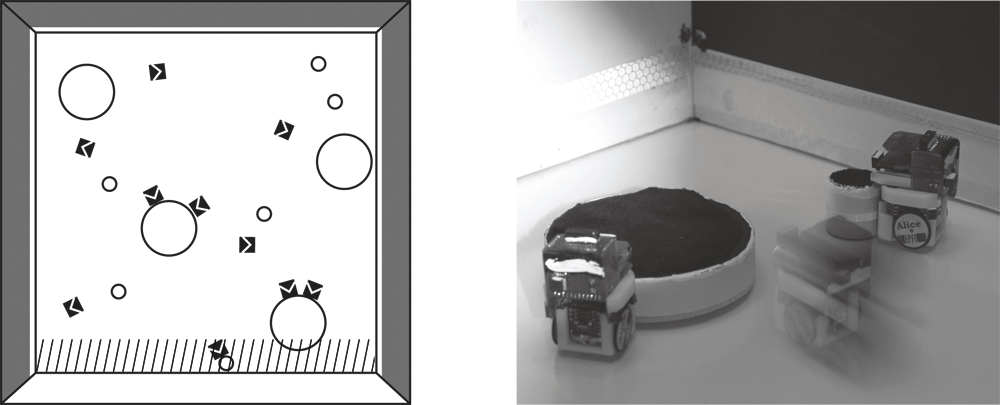
\includegraphics[width=\textwidth]{waibel-fig-3}
\vspace{1ex}
\caption{
Figure 3 from \cite{waibel2009genetic}.
}
\end{figure}

\end{frame}

\begin{frame}{Results}

\begin{figure}
\begin{columns}
\begin{column}{0.7\textwidth}
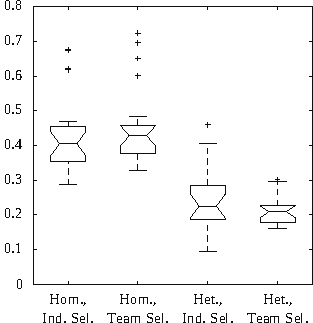
\includegraphics[width=\textwidth]{waibel-fig-9-b}
\end{column}
\begin{column}{0.3\textwidth}
\caption{
Right column of Figure 9 from \cite{waibel2009genetic}.
}
\end{column}
\end{columns}
\end{figure}

\end{frame}

\begin{frame}{Results}


\begin{figure}
\begin{columns}
\begin{column}{0.7\textwidth}
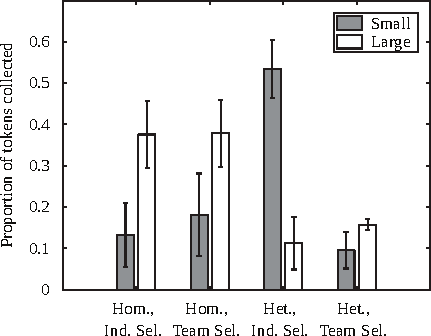
\includegraphics[width=\textwidth]{waibel-fig-10}
\end{column}
\begin{column}{0.3\textwidth}
\caption{
Figure 10 from \cite{waibel2009genetic}.
}
\end{column}
\end{columns}
\end{figure}

\end{frame}

\begin{frame}{Results}

\begin{figure}
\begin{columns}
\begin{column}{0.8\textwidth}
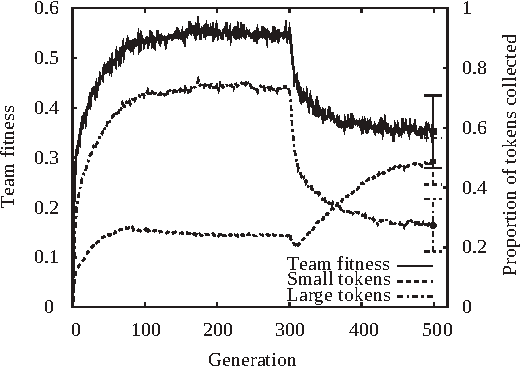
\includegraphics[width=\textwidth]{waibel-fig-12}
\end{column}
\begin{column}{0.2\textwidth}
\caption{
Figure 12 from \cite{waibel2009genetic}.
}
\end{column}
\end{columns}
\end{figure}

\end{frame}

\begin{frame}{Discussion}

\end{frame}
